\section{Metodologia}
\label{sec:metodologia}

O estudo implementa um \textit{pipeline} determinístico em Python~\cite{projeto_github} para reconstruir a rede licitatória e societária do município de Divinópolis/MG no exercício de 2025. O fluxo compreende a higienização dos registros, a construção do grafo multicamada, o enriquecimento dos dados societários e administrativos via QSA, o cálculo de escores para pares co-disputantes e a redução topológica. A Figura~\ref{fig:fluxograma_eixo1} apresenta a organização geral das etapas do módulo analisado.

\begin{figure*}[!t]
\centering
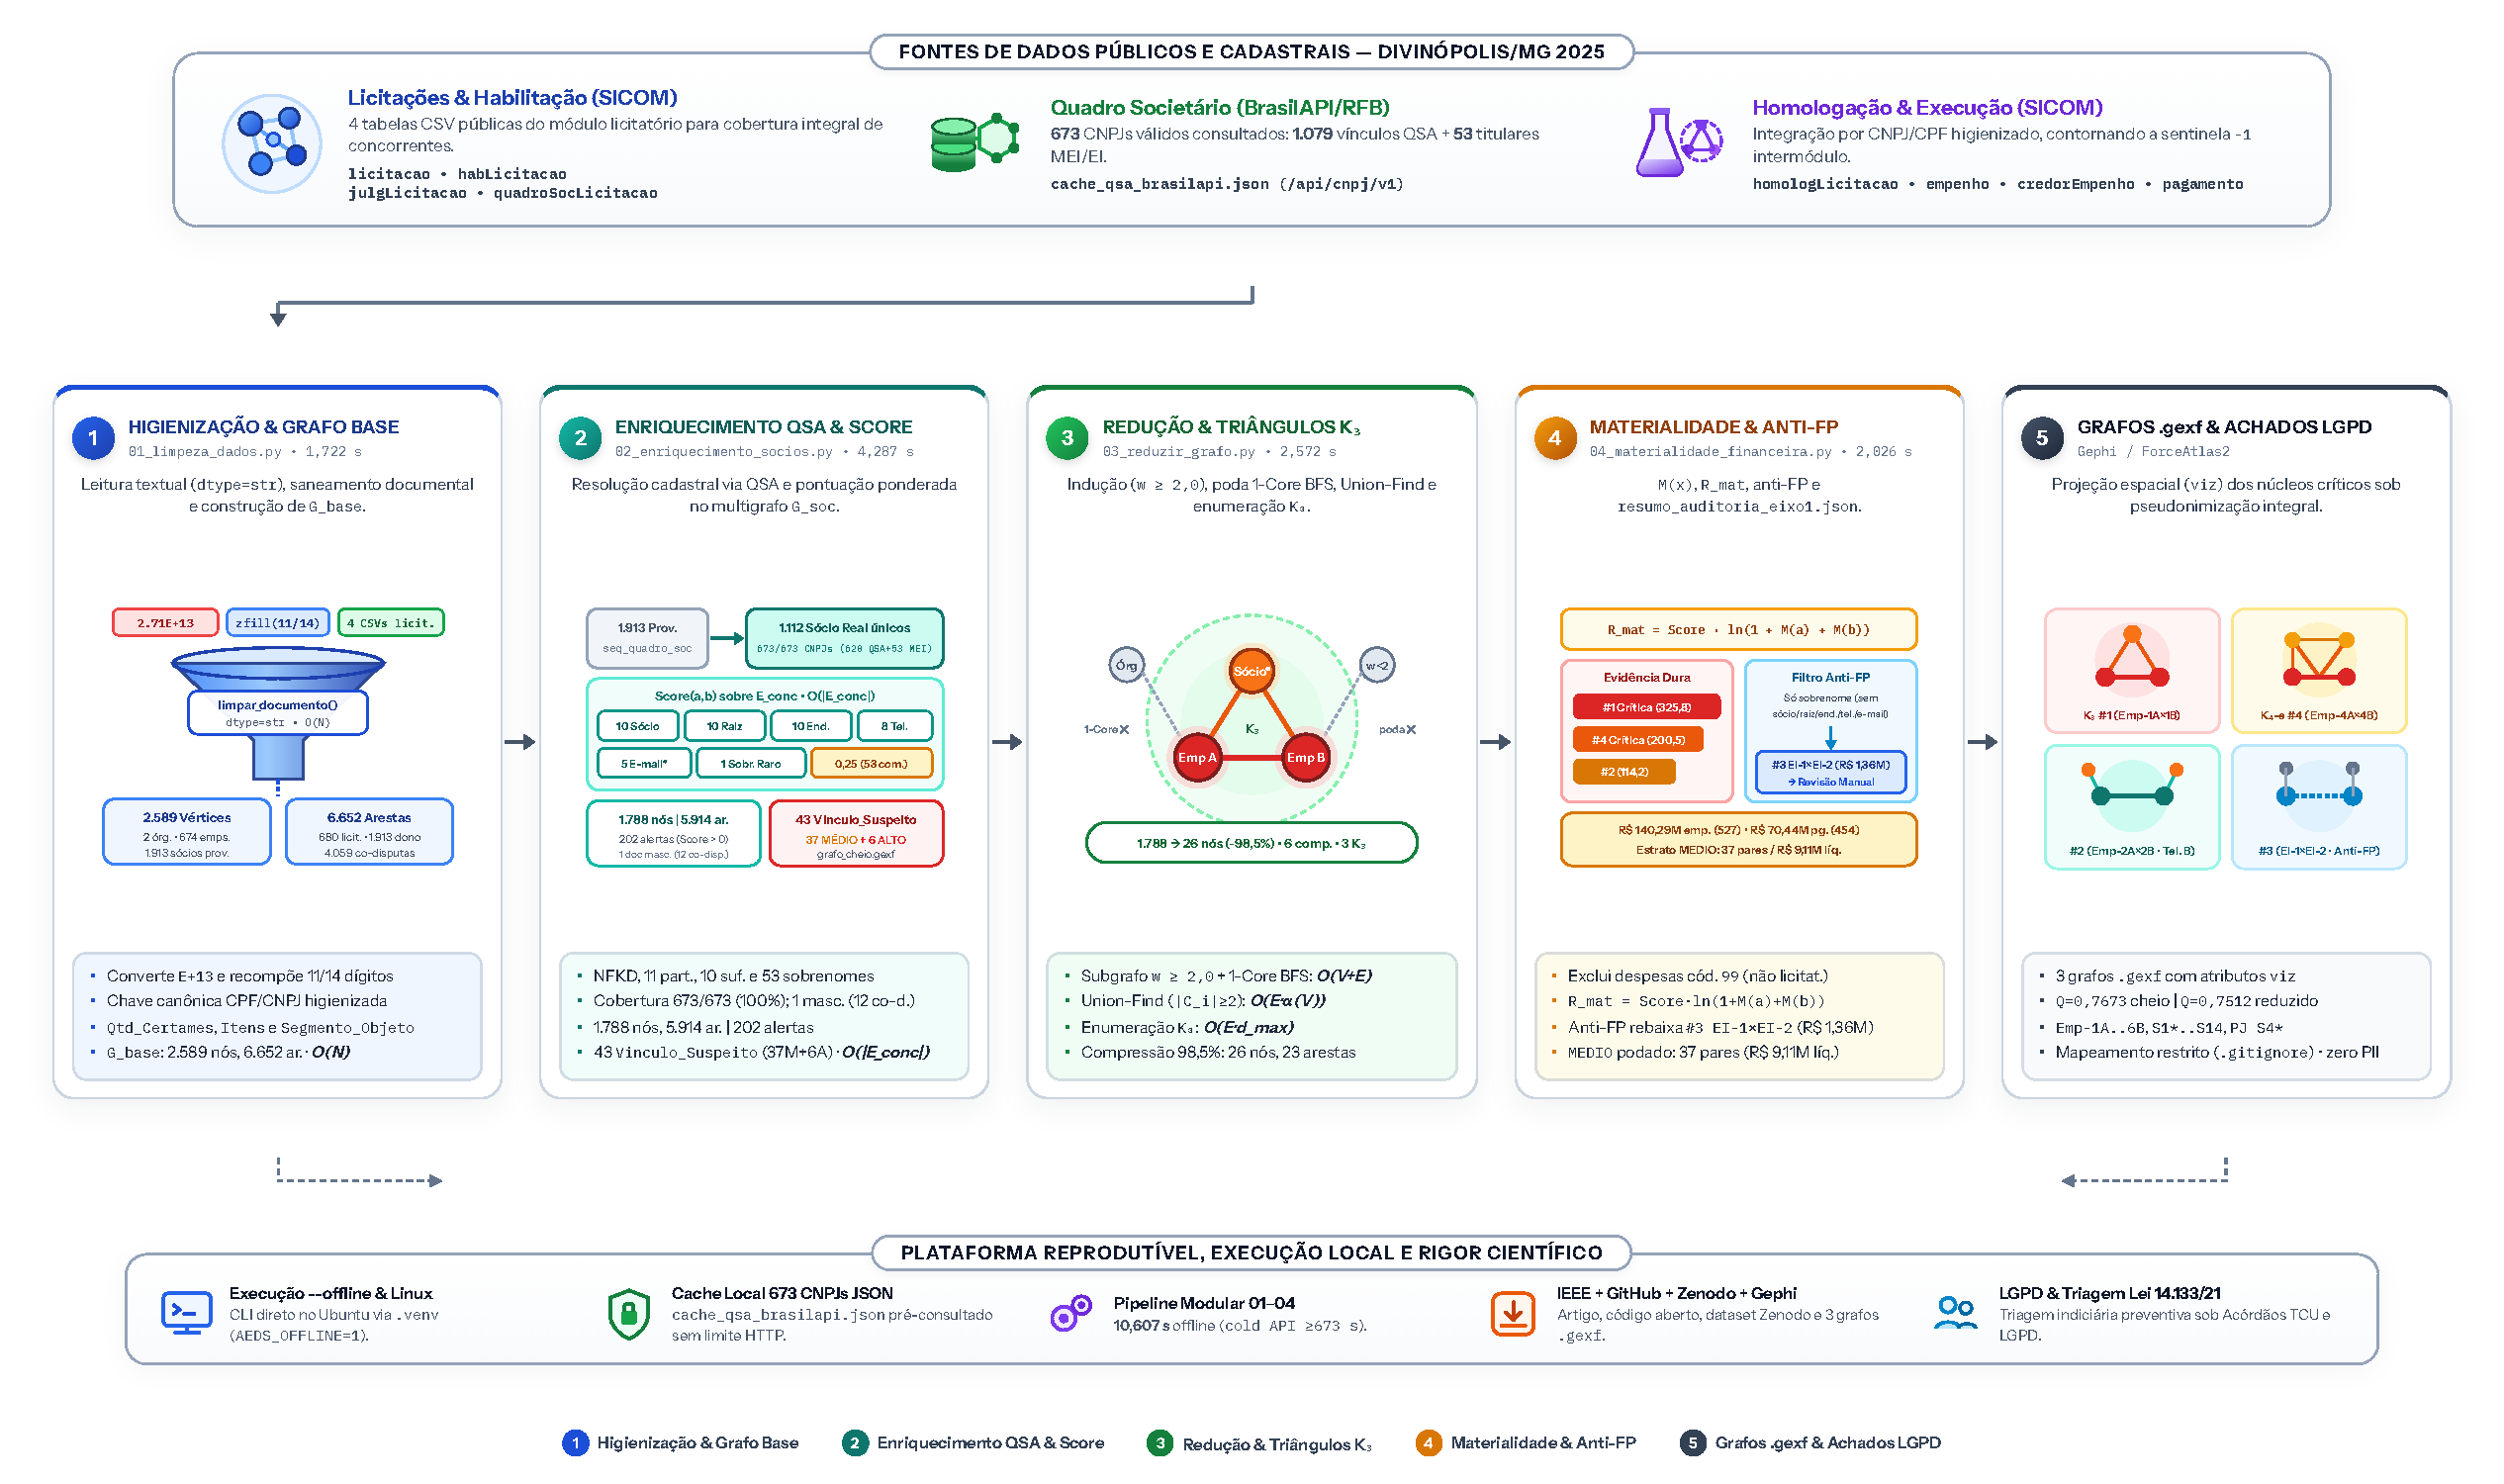
\includegraphics[width=0.93\textwidth, trim= 0 1.3cm 0 0, clip]{figures/fluxograma_eixo1.pdf}
\caption{Fluxograma do módulo de análise de relações societárias e licitatórias. O fluxo contempla as fontes SICOM/TCE-MG e BrasilAPI, a higienização, a construção do grafo, o enriquecimento QSA, a pontuação e a redução topológica.}
\label{fig:fluxograma_eixo1}
\end{figure*}

\subsection{Obtenção e Tratamento de Dados}

Os registros licitatórios provêm das remessas consolidadas de 2025 do município de Divinópolis/MG, identificado pelo código \texttt{3122306}, no Portal de Dados Abertos do TCE-MG~\cite{tce_mg_dados_abertos,tcemg2025in01}. Foram processadas quatro tabelas CSV do módulo \texttt{licitacao}: \texttt{licitacao.csv}, \texttt{habLicitacao.csv}, \texttt{julgLicitacao.csv} e \texttt{quadroSocLicitacao.csv}. Os dados societários foram complementados por consultas ao QSA da Receita Federal via BrasilAPI~\cite{brasilapi2026cnpj}.

A análise exploratória identificou problemas de formatação em documentos fiscais, incluindo perda de zeros à esquerda e conversão indevida para notação científica (por exemplo, \texttt{2.71E+13}). Para evitar alterações decorrentes da interpretação numérica dos identificadores, os arquivos foram carregados como texto e submetidos a uma rotina de saneamento. A rotina remove caracteres de formatação e restaura o comprimento esperado dos documentos: 14 dígitos para CNPJ e 11 dígitos para CPF. Em seguida, foram consolidados os participantes únicos registrados nas fases de habilitação e julgamento.

O cruzamento financeiro entre licitações, contratos, empenhos e pagamentos não é utilizado para produzir os resultados quantitativos apresentados. A inspeção das tabelas indicou preenchimento de chaves estrangeiras intermódulo com o valor sentinela \texttt{-1}, o que impede a associação direta e unívoca entre determinados certames e seus registros de execução orçamentária. Embora existam chaves intramódulo válidas, a reconstrução de uma ligação confiável entre o certame e a despesa executada exige procedimento adicional de integração e validação. Por essa razão, a materialidade financeira não é apresentada como achado deste estudo.

\subsection{Modelagem do Grafo Multicamada}

Após a consolidação dos participantes, a rede é modelada como um grafo heterogêneo multicamada ponderado:
\begin{equation}
  G=(V,E,\tau_V,\tau_E,w),
  \label{eq:grafo_metodologia}
\end{equation}
em que $V$ representa o conjunto de vértices, $E$ o conjunto de arestas, $\tau_V:V\rightarrow\mathcal{T}_V$ identifica o tipo de entidade, $\tau_E:E\rightarrow\mathcal{T}_E$ identifica a camada relacional e $w:E\rightarrow\mathbb{R}_{>0}$ atribui o peso da relação.

\subsubsection{Partições de Vértices}

\begin{itemize}
  \item \textbf{Órgãos públicos:} entidades municipais responsáveis pelos certames;
  \item \textbf{Empresas licitantes:} pessoas jurídicas e pessoas físicas registradas como participantes nas fases de habilitação ou julgamento;
  \item \textbf{Integrantes do QSA (sócios, controladores e administradores):} pessoas físicas e pessoas jurídicas retornadas no campo \texttt{qsa} da BrasilAPI — abrangendo todas as qualificações registradas na Receita Federal (\textit{Sócio-Administrador}, \textit{Sócio}, \textit{Administrador}, \textit{Diretor}, \textit{Conselheiro de Administração}, \textit{Presidente}, entre outras), sem filtragem prévia de papéis administrativos — além de titulares de MEI e empresários individuais extraídos da razão social conforme a regra descrita adiante.
\end{itemize}

\subsubsection{Camadas de Arestas}

\begin{itemize}
  \item \texttt{Participou\_Licitacao}: conecta uma empresa ao órgão responsável pelo certame em que participou;
  \item \texttt{Concorreu\_Contra}: conecta pares de empresas co-disputantes. Operacionalmente, a construção dessa camada combina duas regras aditivas em \texttt{01\_limpeza\_dados.py}: (i) união deduplicada de participantes por par $(\texttt{seq\_licitacao}, \texttt{documento})$ nas tabelas \texttt{habLicitacao.csv} e \texttt{julgLicitacao.csv}, adicionando $+1$ para cada certame compartilhado (\texttt{Qtd\_Certames\_Comuns}); e (ii) agrupamento por \texttt{seq\_item\_licitacao} em \texttt{julgLicitacao.csv}, adicionando $+1$ para cada item disputado em comum (\texttt{Qtd\_Itens\_Comuns}). O peso da aresta, armazenado em \texttt{Peso\_Concorrencia}, corresponde à soma \texttt{Qtd\_Certames\_Comuns} $+$ \texttt{Qtd\_Itens\_Comuns}. Os contadores separados e o segmento do objeto (\texttt{Segmento\_Objeto}) são preservados como metadados para auditoria. Consequentemente, empresas que participaram de itens distintos dentro de um mesmo certame recebem uma aresta com \texttt{Qtd\_Certames\_Comuns} $= 1$ e \texttt{Qtd\_Itens\_Comuns} $= 0$;
  \item \texttt{É\_Dono\_De}: conecta integrantes do QSA (sócios, controladores ou administradores) e titulares de MEI às empresas às quais estão vinculados;
  \item \texttt{Vinculo\_Suspeito}: conecta pares co-disputantes com sobreposição cadastral, onomástica ou de vínculos no QSA acima do limite mínimo de retenção.
\end{itemize}

As relações são armazenadas simetricamente na estrutura computacional de listas de adjacência, embora algumas possuam direção semântica natural. A camada de co-disputa é uma projeção ponderada entre empresas, cuja regra de agregação preserva a distinção entre co-participação por certame e disputa direta por item.

\subsection{Enriquecimento Societário e Escore Multidimensional}

Como os registros do SICOM não disponibilizam todos os identificadores dos integrantes do QSA necessários à análise, realizou-se enriquecimento cadastral mediante consultas à Receita Federal via BrasilAPI~\cite{brasilapi2026cnpj}, com persistência em \textit{cache} local obtido em 14 de novembro de 2026. Por refletir a composição cadastral vigente na data da coleta, a existência de um vínculo no QSA não comprova, isoladamente, que a relação estivesse ativa nas datas específicas dos certames de 2025, exigindo conferência histórica documental nos casos selecionados. Para MEIs e empresários individuais sem QSA formal, o titular foi extraído da razão social mediante remoção de dígitos e pontuações iniciais.

Antes da comparação entre empresas, os atributos cadastrais passaram por regras determinísticas de validação e normalização para evitar que valores ausentes ou inválidos gerem coincidências espúrias:
\begin{itemize}
  \item \textbf{Endereços e telefones:} conversão de logradouro, número, município e UF para ASCII maiúsculo, com descarte completo (retorno vazio) quando o logradouro é genérico (\texttt{RUA}) ou o número é ausente/inválido (\texttt{S/N}, \texttt{SN}, \texttt{0} ou vazio); para telefones, manutenção apenas de dígitos numéricos com comprimento $\ge 8$ que não iniciem por \texttt{0000};
  \item \textbf{Correio eletrônico:} conversão para minúsculas com verificação da presença de \texttt{@} e descarte de endereços contendo qualquer um dos cinco termos associados a escritórios terceirizados (\texttt{contabil}, \texttt{contador}, \texttt{contabilidade}, \texttt{assessoria}, \texttt{escritorio});
  \item \textbf{Onomástica:} normalização dos nomes de integrantes do QSA classificados como pessoa física (ou titular de MEI) para ASCII maiúsculo sem pontuação, remoção do primeiro prenome (\texttt{tokens[1:]}), de tokens unitários ($\le 1$ caractere), de 11 preposições/partículas (\texttt{DE}, \texttt{DA}, \texttt{DO}, \texttt{DAS}, \texttt{DOS}, \texttt{E}, \texttt{D}, \texttt{DI}, \texttt{DEL}, \texttt{VAN}, \texttt{VON}) e de 10 sufixos genealógicos (\texttt{FILHO}, \texttt{FILHA}, \texttt{JUNIOR}, \texttt{JR}, \texttt{NETO}, \texttt{NETA}, \texttt{SOBRINHO}, \texttt{SOBRINHA}, \texttt{SEGUNDO}, \texttt{TERCEIRO}).
\end{itemize}

Para reduzir falsos positivos associados a sobrenomes frequentes, adotou-se uma ponderação discreta inspirada no princípio de frequência inversa. Cada sobrenome compartilhado $n$ recebe peso
\begin{equation}
w(n)=
\begin{cases}
0{,}25, & \text{se } n \in \mathcal{T}_{\mathrm{comum}};\\
1{,}00, & \text{caso contrário},
\end{cases}
\end{equation}
em que $\mathcal{T}_{\mathrm{comum}}$ é a lista versionada e determinística de 53 sobrenomes brasileiros frequentes (\texttt{SOBRENOMES\_COMUNS}) disponibilizada no repositório do código~\cite{projeto_github}.

Para cada par de empresas co-disputantes $(a,b)$, o escore de vínculo é definido por
\begin{equation}
\begin{aligned}
s(a,b)=\;&10|S(a)\cap S(b)|\\
&+10[\mathrm{raiz}(a)=\mathrm{raiz}(b)]\\
&+10[\mathrm{end}(a)=\mathrm{end}(b)]\\
&+8[\mathrm{tel}(a)=\mathrm{tel}(b)]\\
&+5[\mathrm{email}(a)=\mathrm{email}(b)]\\
&+\sum_{n\in N(a)\cap N(b)}w(n),
\end{aligned}
\label{eq:escore_vinculo}
\end{equation}
em que $S(x)$ representa o conjunto de nomes normalizados e não vazios dos integrantes do QSA (sócios ou administradores) vinculados à empresa $x$; $\mathrm{raiz}(x)$ representa os oito primeiros dígitos de CNPJs válidos de 14 dígitos; $\mathrm{end}(x)$, $\mathrm{tel}(x)$ e $\mathrm{email}(x)$ representam os atributos cadastrais validados; e $N(x)$ representa o conjunto de sobrenomes extraídos. O operador $[P]\in\{0,1\}$ assume valor $1$ se, e somente se, a condição $P$ é verdadeira \textbf{e ambos os atributos comparados são válidos e não vazios}, assumindo $0$ caso contrário.

A recorrência de co-disputa, armazenada em \texttt{Peso\_Concorrencia}, não integra a soma de $s(a,b)$; ela é mantida como atributo relacional e utilizada como critério auxiliar de ordenação dos alertas. Os pares com escore positivo são agrupados em três \textbf{faixas heurísticas do escore de triagem}: faixa \texttt{BAIXO}, para $0<s(a,b)<1{,}00$; faixa \texttt{MEDIO}, para $1{,}00\leq s(a,b)<2{,}00$; e faixa \texttt{ALTO}, para $s(a,b)\geq2{,}00$ ou presença de vínculo direto no QSA, mesma raiz de CNPJ, mesmo endereço ou mesmo telefone. Como os pesos e os cortes $\theta=1{,}00$ e $\theta=2{,}00$ são heurísticos e não passaram por calibração empírica com casos rotulados ou análise de sensibilidade, essas categorias não representam probabilidades validadas de irregularidade; em particular, um par sem vínculo cadastral ou societário direto pode atingir $s(a,b)=2{,}00$ exclusivamente pela coincidência de dois sobrenomes ausentes de $\mathcal{T}_{\mathrm{comum}}$. Na base analisada, os pares da faixa \texttt{BAIXO} são excluídos da camada \texttt{Vinculo\_Suspeito}; os pares das faixas \texttt{MEDIO} e \texttt{ALTO} são mantidos, totalizando 43 arestas. A redução topológica posterior utiliza o limiar numérico $\theta=2{,}00$.

\subsection{Redução Topológica e Identificação de Motivos $K_3$}

A redução tem por objetivo remover as relações de participação institucional e de concorrência ordinária que não integram o domínio prioritário da análise, preservando as arestas suspeitas de maior escore e as relações societárias incidentes às empresas envolvidas. O procedimento é composto pelas etapas seguintes.

\begin{enumerate}
  \item \textbf{Filtragem por predicado de arestas:} define-se $V_{\mathrm{suspeito}}$ como o conjunto das empresas incidentes em arestas \texttt{Vinculo\_Suspeito} com peso $s(a,b)\geq\theta$, em que $\theta=2{,}00$. Retêm-se as arestas que satisfazem
  \begin{equation}
  \begin{aligned}
  \mathcal{P}(u,v,t,w)\iff&
  \big(t=\mathrm{sus}\land w\geq\theta\big)\\
  &\lor\big(t=\mathrm{prop}\land
  (u\in V_{\mathrm{suspeito}}\\
  &\hspace{3.7em}\lor v\in V_{\mathrm{suspeito}})\big),
  \end{aligned}
  \label{eq:predicado_reducao}
  \end{equation}
  em que $\mathrm{sus}$ identifica a camada \texttt{Vinculo\_Suspeito} e $\mathrm{prop}$ identifica a camada \texttt{É\_Dono\_De}.
  A varredura das listas de adjacência possui custo $O(|V|+|E|)$. Como a seleção é feita por predicado de arestas, denomina-se esta etapa \textit{subgrafo filtrado por arestas}, e não subgrafo induzido por vértices.

  \item \textbf{Remoção de vértices isolados:} após a filtragem, removem-se os vértices cujo grau é zero. O resultado corresponde ao $1$-core do grafo filtrado. Essa operação pode ser executada por uma varredura de vértices em $O(|V|+|E|)$; a menção a uma fila ou BFS deve ser entendida apenas como detalhe de implementação, não como requisito matemático do $1$-core.

  \item \textbf{Componentes conexas por Union-Find:} aplica-se a estrutura de conjuntos disjuntos com compressão de caminho e união por posto. Para a inicialização dos vértices e a sequência de operações sobre as arestas, o custo amortizado é
  \begin{equation}
    O\big((|V|+|E|)\alpha(|V|)\big),
  \end{equation}
  em que $\alpha$ representa a função inversa de Ackermann. São mantidas as componentes não triviais, com $|C_i|\geq2$.

  \item \textbf{Enumeração dos motivos triangulares:} para cada aresta suspeita $(a,b)$ entre empresas, calcula-se a interseção
  \begin{equation}
    \mathrm{Donos}(a)\cap\mathrm{Donos}(b),
  \end{equation}
  em que $\mathrm{Donos}(x)$ é o conjunto de integrantes do QSA (sócios, controladores ou administradores) associados à empresa $x$ na camada \texttt{É\_Dono\_De}. Cada elemento $s$ dessa interseção forma o motivo tipado $\{(s,a),(s,b),(a,b)\}$: duas arestas \texttt{É\_Dono\_De} e uma aresta \texttt{Vinculo\_Suspeito}. A enumeração ocorre na representação agregada multicamada; a camada bipartida do QSA, isoladamente, não contém triângulos.
\end{enumerate}

\subsection{Proteção de Dados e Limites Éticos}

Os resultados são apresentados com identificadores pseudonimizados. Os vértices de empresas, empresários individuais e sócios recebem rótulos artificiais; nomes civis, CPFs e CNPJs não são reproduzidos nas tabelas e figuras. Endereços e telefones coincidentes são descritos por rótulos genéricos, sem exposição dos valores completos. A chave de correspondência, quando necessária à auditoria autorizada, deve permanecer separada do material público e sob controle de acesso.

A pseudonimização é uma medida de redução de exposição, mas não deve ser descrita como anonimização integral. A divulgação deve observar os princípios de finalidade, adequação e necessidade da LGPD~\cite{brasil2018lgpd}. Por fim, nenhum escore ou motivo topológico deve ser interpretado isoladamente como comprovação de ilícito; os achados demandam validação documental e contextual.
